\partie{TROISIÈME PARTIE}{PLOMBERIE SANITAIRE}

\section{Généralités sur la plomberie sanitaire}

\subsection{Définition et rôle}
La plomberie sanitaire regroupe l'ensemble des installations qui assurent, dans un bâtiment,
l'\textbf{alimentation en eau} des appareils sanitaires (eau froide et eau chaude) et
l'\textbf{évacuation des eaux usées et des eaux vannes} vers le réseau d'assainissement. Elle
doit garantir à chaque point de puisage un débit et une pression suffisants, une eau de
qualité, l'absence de bruit et de fuite, et la sécurité des usagers. En France, ces
installations sont encadrées par le NF DTU~60.1 pour la mise en œuvre et par le NF DTU~60.11
pour les règles de calcul \cite{dtu601,dtu6011}. Ces documents servent couramment de
référence technique au Cameroun.

\subsection{Constitution d'une installation}
Une installation de plomberie sanitaire comprend les éléments suivants
(figure~\ref{fig:principe}) :
\begin{itemize}
  \item le \textbf{branchement} au réseau public, avec le compteur, une vanne d'arrêt et un
        clapet anti-retour ;
  \item le cas échéant, un \textbf{réservoir de stockage (bâche)} et un \textbf{surpresseur},
        lorsque la pression du réseau public est insuffisante pour desservir les étages ;
  \item la \textbf{distribution d'eau froide} (EF) : colonnes montantes, puis distribution par
        étage et par logement ;
  \item la \textbf{production d'eau chaude sanitaire} (ECS) : chauffe-eau électrique,
        chaudière ou système solaire, et la distribution d'ECS ;
  \item les \textbf{organes de régulation et de contrôle} : réducteurs de pression, manomètres,
        vannes d'isolement, purges ;
  \item les \textbf{appareils sanitaires} : lavabos, douches, WC, éviers ;
  \item les \textbf{évacuations} : eaux usées (EU), eaux vannes (EV) et leur ventilation.
\end{itemize}

\begin{figure}[H]\centering
% Schéma de principe : branchement -> bâche -> surpresseur -> colonnes EF/ECS -> étages -> évacuations
\begin{tikzpicture}[font=\scriptsize, >=Stealth,
  eq/.style={draw=vertnuit, fill=vertclair, rounded corners=2pt, align=center, minimum height=8mm, inner sep=3pt},
  app/.style={draw=gray!70, fill=white, align=center, minimum width=10mm, minimum height=5mm, inner sep=1pt},
  ef/.style={blue!70!black, line width=1.2pt},
  ecs/.style={red!75!black, line width=1.2pt},
  eu/.style={brown!70!black, line width=1.6pt, dashed}]
  % Réseau public et branchement
  \node[eq] (pub) at (0,0) {Réseau\\public};
  \node[eq, right=6mm of pub] (cpt) {Compteur\\+ clapet};
  \node[eq, right=6mm of cpt] (bache) {Bâche\\(stockage)};
  \node[eq, right=6mm of bache] (surp) {Surpresseur};
  \draw[ef,->] (pub) -- (cpt);
  \draw[ef,->] (cpt) -- (bache);
  \draw[ef,->] (bache) -- (surp);
  % Colonnes
  \coordinate (cEF) at (8.6,0);
  \coordinate (cECS) at (9.4,0);
  \draw[ef] (surp) -- (cEF);
  \draw[ef,->] (cEF) -- ++(0,5.6) node[above left, inner sep=1pt] {Colonne EF};
  % Production ECS
  \node[eq, fill=red!10] (ce) at (11.2,0.9) {Production\\ECS};
  \draw[ef,->] (cEF |- ce.west) -- (ce.west);
  \draw[ecs] (ce.north) |- (cECS |- 1.8,1.8);
  \draw[ecs,->] (cECS |- 1.8,1.8) -- (cECS |- 5.6,5.6) node[above right, inner sep=1pt] {Colonne ECS};
  % Étages
  \foreach \y/\n/\i in {2.6/R+1/a, 3.8/R+2/b, 5.0/R+N/c} {
    \draw[gray!50] (-0.3,\y-0.45) -- (12.6,\y-0.45);
    \node[anchor=west, gray] at (-0.3,\y) {\n};
    \node[eq, fill=white, minimum height=6mm] (rp\i) at (7.2,\y-0.08) {Réducteur\\+ manomètre};
    \draw[ef,->] (cEF |- rp\i.east) -- (rp\i.east);
    \node[app] (lav\i) at (1.6,\y) {Lavabo};
    \node[app] (dou\i) at (3.0,\y) {Douche};
    \node[app] (wc\i) at (4.4,\y) {WC};
    \draw[ef,->] (rp\i.west) -- (wc\i.east);
    \draw[ecs] (cECS |- 0,\y+0.42) -- (2.2,\y+0.42) -- (2.2,\y+0.3);
    \draw[eu] (4.4,\y-0.25) -- (4.4,\y-0.38) -- (0.75,\y-0.38); \draw[eu] (1.6,\y-0.25) -- (1.6,\y-0.38); \draw[eu] (3.0,\y-0.25) -- (3.0,\y-0.38);
  }
  % Chute EU/EV
  \draw[eu,->] (0.75,4.62) -- (0.75,1.1) node[right, text=brown!70!black] {Chute EU/EV vers l'égout};
  % Légende
  \begin{scope}[shift={(0,-1.6)}]
    \draw[ef] (0,0) -- (0.6,0); \node[anchor=west] at (0.7,0) {Eau froide (EF)};
    \draw[ecs] (3.2,0) -- (3.8,0); \node[anchor=west] at (3.9,0) {Eau chaude sanitaire (ECS)};
    \draw[eu] (7.4,0) -- (8.0,0); \node[anchor=west] at (8.1,0) {Évacuations EU/EV};
  \end{scope}
\end{tikzpicture}

\caption{schéma de principe d'une installation de plomberie sanitaire d'immeuble}\label{fig:principe}
\end{figure}

Le détail de la distribution à l'intérieur d'un logement est donné en
\hyperref[ann:schema]{annexe~1}.

\subsection{Matériaux des canalisations}
Le choix du matériau dépend de l'usage (eau froide, eau chaude, évacuation), de la pression,
de la température et du coût. Le tableau~\ref{tab:materiaux} compare les principaux matériaux
rencontrés sur les chantiers.

\begin{table}[H]\centering
\caption{comparaison des matériaux de canalisation}\label{tab:materiaux}
\begin{tabularx}{\textwidth}{>{\bfseries}p{2.3cm} p{3.2cm} Y Y}
\toprule
\entete Matériau & Usage & Avantages & Limites \\
\midrule
PPR & EF et ECS & Assemblage par polyfusion sans colle, bonne tenue en température, durable, économique & Dilatation importante, nécessite un outillage spécifique \\
PER & EF et ECS (distribution) & Souple, pose rapide en nourrice, peu de raccords & Sensible aux UV, raccords à sertir ou à glissement \\
PE & Branchement enterré & Résistant, soudable, adapté aux grandes longueurs & Pas d'eau chaude, réservé à l'extérieur \\
Cuivre & EF, ECS, froid & Robuste, résistant à la chaleur, compatible avec les fluides frigorigènes & Coût élevé, brasage, risque de vol \\
PVC & Évacuations EU/EV & Léger, économique, collage simple & Pas d'eau chaude sous pression, fragile aux chocs \\
\bottomrule
\end{tabularx}
\end{table}

Sur le chantier, la distribution d'eau froide et d'eau chaude est réalisée en \textbf{PPR},
et les évacuations en \textbf{PVC}.

\subsection{Exigences de pression et de vitesse}
Pour éviter les nuisances sonores, les coups de bélier et l'usure prématurée de la
robinetterie, la vitesse de l'eau doit rester limitée. Le NF DTU~60.11 retient les valeurs du
tableau~\ref{tab:vitesses} \cite{dtu6011,caleffiReducteurs}.

\begin{table}[H]\centering
\caption{vitesses maximales de l'eau dans les canalisations}\label{tab:vitesses}
\begin{tabular}{l c}
\toprule
\entete \textbf{Emplacement} & \textbf{Vitesse maximale} \\
\midrule
Sous-sol et locaux techniques & \SI{2}{\metre\per\second} \\
Colonnes montantes & \SI{1,5}{\metre\per\second} \\
Distribution d'étage et branchements & \SI{1}{\metre\per\second} \\
\bottomrule
\end{tabular}
\end{table}

À l'inverse, la pression doit être suffisante au point de puisage le plus défavorisé, en
général le plus haut et le plus éloigné. Une pression résiduelle d'environ \SI{1}{bar} y est
recherchée. Aux étages bas, la pression ne doit pas être excessive : on la limite par des
réducteurs de pression, couramment réglés autour de \SI{3}{bar} \cite{caleffiReducteurs}.

\section{Présentation du chantier}

\subsection{Situation et description du bâtiment}
Le chantier \InfoChantier{} est situé à \InfoChantierVille. Il s'agit d'un immeuble de type
\InfoChantierNiveaux{} à usage d'hôtel et de logements, dont \InfoEntrepriseSigle{} réalise
notamment le lot plomberie sanitaire. La figure~\ref{fig:facade} en présente la façade
principale. \AC{Maître d'ouvrage, maître d'œuvre, nombre de chambres et de logements, état
d'avancement à l'arrivée du stagiaire.}

\figureimg{img/fig_facade_chantier}{0.7\textwidth}{façade principale du bâtiment du chantier}{fig:facade}

\subsection{Principe de distribution adopté}
L'eau du réseau public est stockée dans une bâche au sous-sol. Un surpresseur alimente une
\textbf{colonne montante} d'eau froide qui dessert tous les étages. À chaque étage, une
nourrice distribue l'eau froide vers les chambres. L'eau chaude est produite par des
chauffe-eau ou par une production centralisée, selon les zones.

Le surpresseur doit fournir une pression suffisante pour le dernier étage. Les étages bas
reçoivent donc une pression plus forte : c'est pourquoi des \textbf{réducteurs de pression}
équipés de \textbf{manomètres} sont installés en pied de distribution d'étage
(figure~\ref{fig:colonne}). Ce principe sera justifié par le calcul de la section suivante.

\begin{figure}[H]\centering
% Colonne montante R+10 : pression décroissante, réducteurs aux étages RDC à R+4
\begin{tikzpicture}[font=\scriptsize, >=Stealth, y=0.48cm]
  \draw[blue!70!black, line width=2pt] (0,0) -- (0,10.6);
  \node[draw=vertnuit, fill=vertclair, rounded corners=2pt, align=center] at (0,-1.1)
       {Surpresseur\\ \SI{4,3}{bar}};
  \foreach \k/\p in {0/4{,}3,1/4{,}0,2/3{,}7,3/3{,}4,4/3{,}1,5/2{,}8,6/2{,}5,7/2{,}2,8/1{,}9,9/1{,}6,10/1{,}3} {
    \draw[gray!40] (-2.6,\k) -- (6.2,\k);
    \pgfmathtruncatemacro{\red}{\k<5 ? 1 : 0}
    \ifnum\k=0 \node[anchor=east, gray] at (-1.4,\k+0.35) {RDC};
    \else \node[anchor=east, gray] at (-1.4,\k+0.35) {R+\k}; \fi
    \node[anchor=east] at (-0.15,\k+0.35) {\p~bar};
    \ifnum\red=1
      \draw[blue!70!black, line width=1pt] (0,\k+0.35) -- (1.2,\k+0.35);
      \node[draw=acompleter, fill=acompleter!15, minimum size=3.2mm, inner sep=0pt] at (1.4,\k+0.35) {};
      \draw[blue!70!black, line width=1pt,->] (1.6,\k+0.35) -- (3.0,\k+0.35)
           node[right, black] {3,0 bar (réglé)};
    \else
      \draw[blue!70!black, line width=1pt,->] (0,\k+0.35) -- (3.0,\k+0.35)
           node[right, black] {\p~bar};
    \fi
  }
  \node[draw=acompleter, fill=acompleter!15, minimum size=3.2mm, inner sep=0pt] at (-2.2,-3.2) {};
  \node[anchor=west] at (-2.0,-3.2) {Réducteur de pression + manomètre (étages où $P > 3$~bar)};
\end{tikzpicture}

\caption{principe de la colonne montante et des réducteurs de pression d'étage}\label{fig:colonne}
\end{figure}

\section{Étude de cas : dimensionnement d'une colonne d'eau froide}

Cette section applique la méthode du NF DTU~60.11 \cite{dtu6011} à un exemple représentatif du
chantier. Elle illustre le lien entre la théorie vue en formation et la pratique du chantier.

\subsection{Hypothèses}
\begin{itemize}
  \item Immeuble R+10, hauteur d'étage \SI{3}{\metre}, soit \SI{30}{\metre} entre le pied de
        colonne et le dernier niveau ;
  \item 4 chambres par étage, desservies par la même colonne, soit 40 chambres ;
  \item chaque chambre comporte un lavabo, une douche et un WC à réservoir, soit 3 appareils ;
  \item usage hôtelier : coefficient de majoration $C_m = 1{,}25$ \cite{caleffiReducteurs,xpairDebit} ;
  \item canalisations en PPR PN20 (dimensions extérieures × épaisseur).
\end{itemize}

\subsection{Débits de base}
Le débit de base est le débit minimal à assurer à chaque appareil. Les valeurs retenues sont
celles du NF DTU~60.11 \cite{dtu6011,clageDebits,caleffiDebits}.

\begin{table}[H]\centering
\caption{débits de base des appareils d'une chambre}\label{tab:debits}
\begin{tabular}{l c c c}
\toprule
\entete \textbf{Appareil} & \textbf{Débit de base (L/s)} & \textbf{Nombre} & \textbf{Total (L/s)} \\
\midrule
Lavabo & 0,20 & 1 & 0,20 \\
Douche & 0,20 & 1 & 0,20 \\
WC à réservoir & 0,12 & 1 & 0,12 \\
\midrule
\textbf{Chambre} & & \textbf{3} & \textbf{0,52} \\
\bottomrule
\end{tabular}
\end{table}

\subsection{Coefficient de simultanéité et débit probable}
Tous les appareils ne fonctionnent pas en même temps. Le NF DTU~60.11 introduit un coefficient
de simultanéité $y$, fonction du nombre $N$ d'appareils desservis, majoré selon l'usage
\cite{dtu6011,caleffiReducteurs} :
\begin{equation}
  y = \frac{0{,}8}{\sqrt{N-1}} \times C_m
  \qquad\text{et}\qquad
  Q_p = y \times \sum Q_b
\end{equation}
où $Q_p$ est le débit probable et $\sum Q_b$ la somme des débits de base.

\textbf{Distribution d'un étage} (4 chambres, $N = 12$) :
\[
  \sum Q_b = 4 \times 0{,}52 = \SI{2,08}{L/s}, \quad
  y = \frac{0{,}8}{\sqrt{11}} \times 1{,}25 = 0{,}302, \quad
  Q_p = 0{,}302 \times 2{,}08 \approx \SI{0,63}{L/s}
\]

\textbf{Colonne montante} (40 chambres, $N = 120$) :
\[
  \sum Q_b = 40 \times 0{,}52 = \SI{20,8}{L/s}, \quad
  y = \frac{0{,}8}{\sqrt{119}} \times 1{,}25 = 0{,}092, \quad
  Q_p = 0{,}092 \times 20{,}8 \approx \SI{1,91}{L/s}
\]

\subsection{Choix des diamètres}
Le diamètre intérieur minimal se déduit de la vitesse maximale admise :
\begin{equation}
  Q = V \times \frac{\pi D^2}{4}
  \quad\Longrightarrow\quad
  D_{\min} = \sqrt{\frac{4\,Q_p}{\pi\,V_{\max}}}
\end{equation}

\begin{table}[H]\centering
\caption{résultats du dimensionnement}\label{tab:dimensionnement}
\small
\begin{tabular}{l c c c c c}
\toprule
\entete \textbf{Tronçon} & $\boldsymbol{Q_p}$ \textbf{(L/s)} & $\boldsymbol{V_{\max}}$ \textbf{(m/s)} & $\boldsymbol{D_{\min}}$ \textbf{(mm)} & \textbf{Tube PPR} & \textbf{V (m/s)} \\
\midrule
Étage & 0,63 & 1,0 & 28,3 & 50 × 8,3 (Di 33,4) & 0,72 \\
Colonne & 1,91 & 1,5 & 40,2 & 63 × 10,5 (Di 42,0) & 1,38 \\
\bottomrule
\end{tabular}
\end{table}

Les branchements individuels des appareils sont réalisés en tube de \SI{20}{mm} et en
flexibles, conformément aux prescriptions des fabricants de robinetterie.

\subsection{Pertes de charge et pression nécessaire}
Les pertes de charge linéaires dans la colonne sont estimées par la formule de Flamant, usuelle
pour les tubes lisses en matière plastique :
\begin{equation}
  J = 0{,}00092 \, \frac{V^{1,75}}{D^{1,25}}
  = 0{,}00092 \times \frac{1{,}38^{1,75}}{0{,}042^{1,25}}
  \approx \SI{0,085}{\metre\per\metre}
\end{equation}
Sur une longueur développée de \SI{33}{\metre}, majorée de \SI{20}{\percent} pour les pertes
singulières (coudes, tés, vannes), on obtient environ \SI{3,4}{\metre} de colonne d'eau. La
pression minimale en pied de colonne vaut alors :
\[
  H_{\min} = \underbrace{30}_{\text{hauteur}} + \underbrace{3{,}4}_{\text{pertes}}
  + \underbrace{10}_{\text{pression résiduelle}} \approx \SI{43}{\metre}
  \;\text{de colonne d'eau, soit environ}\; \SI{4,3}{bar}
\]

\subsection{Justification des réducteurs de pression}
Avec \SI{4,3}{bar} en pied de colonne, la pression statique décroît d'environ \SI{0,3}{bar}
par étage. Le tableau~\ref{tab:pressions} montre que les étages bas dépassent la valeur de
réglage de \SI{3}{bar}. Les réducteurs de pression y sont indispensables. Le rapport de réduction
reste inférieur à 3:1, ce qui évite le risque de cavitation dans le réducteur
\cite{caleffiReducteurs}.

\begin{table}[H]\centering
\caption{pression disponible par niveau}\label{tab:pressions}
\begin{tabular}{l c c c c c c c}
\toprule
\entete \textbf{Niveau} & RDC & R+1 & R+2 & R+3 & R+4 & R+5 & R+10 \\
\midrule
Pression (bar) & 4,3 & 4,0 & 3,7 & 3,4 & 3,1 & 2,8 & 1,3 \\
Réducteur nécessaire & oui & oui & oui & oui & oui & non & non \\
\bottomrule
\end{tabular}
\end{table}

Ce calcul confirme les observations faites sur le chantier (deuxième partie). Il explique la
place importante prise par le montage des réducteurs de pression dans notre planning.

\section{Matériaux et matériels utilisés}

Les principaux matériaux et matériels utilisés sur le chantier sont présentés ci-après.

\begin{figure}[H]\centering
\begin{minipage}{0.48\textwidth}\centering
  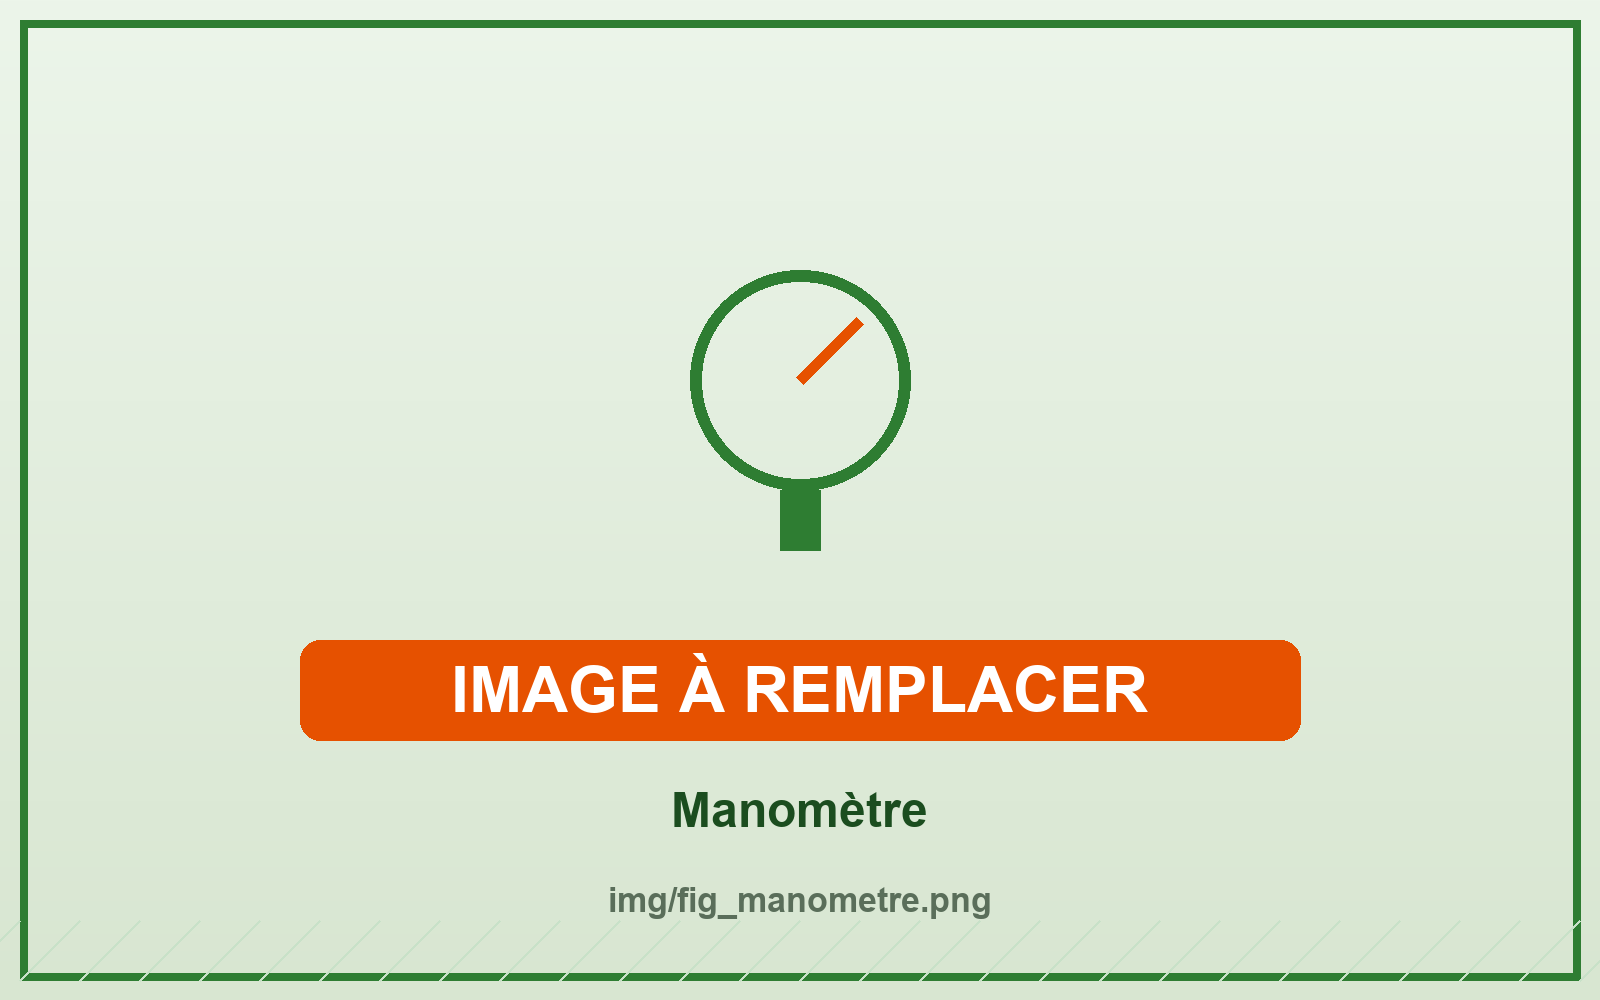
\includegraphics[width=\linewidth]{img/fig_manometre}
  \caption{manomètre}\label{fig:manometre}
\end{minipage}\hfill
\begin{minipage}{0.48\textwidth}\centering
  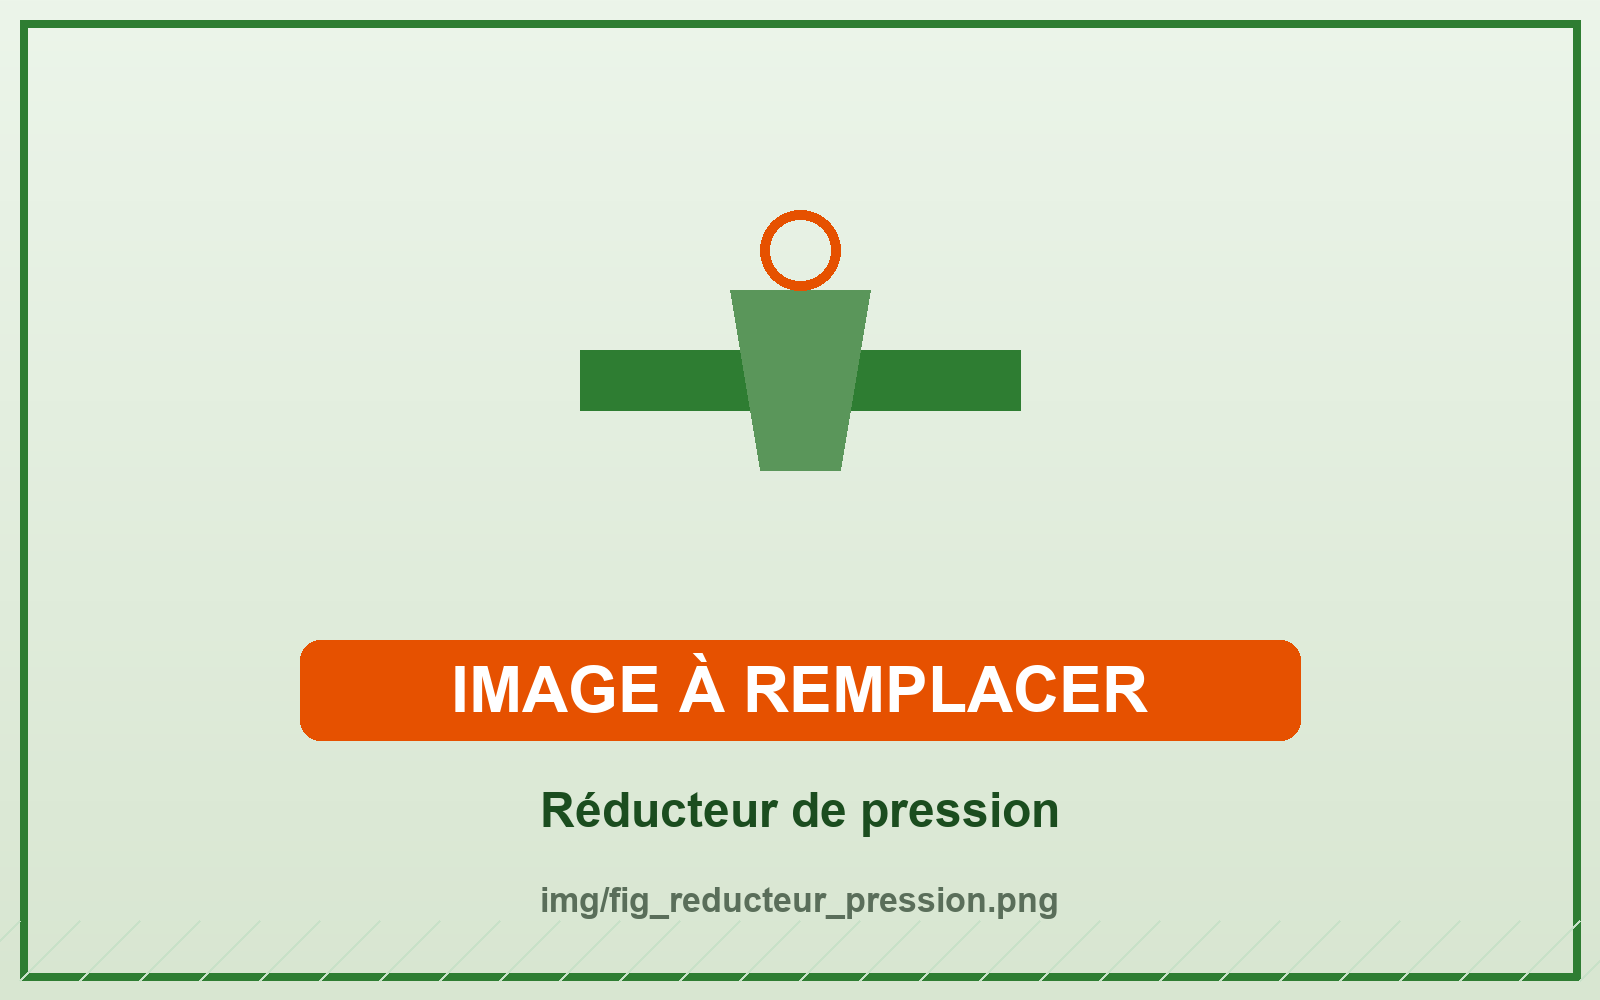
\includegraphics[width=\linewidth]{img/fig_reducteur_pression}
  \caption{réducteur de pression}\label{fig:reducteur}
\end{minipage}
\end{figure}

\begin{itemize}
  \item \textbf{Manomètre} (figure~\ref{fig:manometre}) : il indique la pression de l'eau dans
        le circuit, en bar. Monté en aval du réducteur, il permet de contrôler le réglage.
  \item \textbf{Réducteur de pression} (figure~\ref{fig:reducteur}) : il abaisse et stabilise
        la pression en aval, quelle que soit la pression amont, pour protéger la robinetterie et
        limiter la consommation.
\end{itemize}

\begin{figure}[H]\centering
\begin{minipage}{0.31\textwidth}\centering
  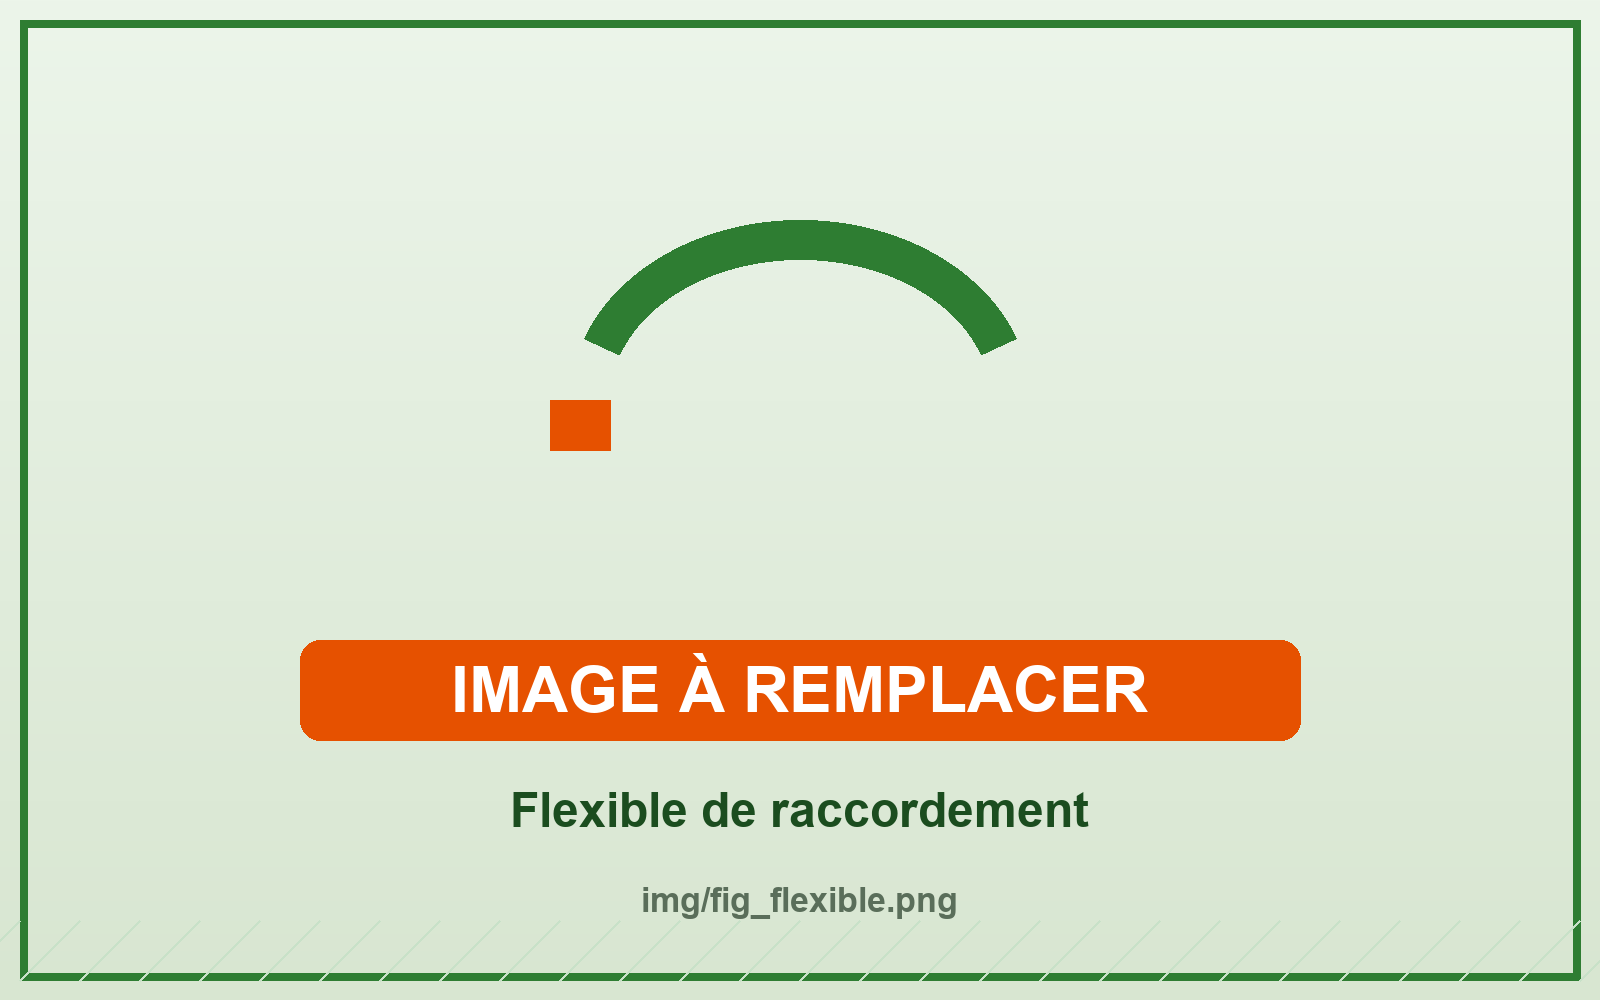
\includegraphics[width=\linewidth]{img/fig_flexible}
  \caption{flexible de raccordement}\label{fig:flexible}
\end{minipage}\hfill
\begin{minipage}{0.31\textwidth}\centering
  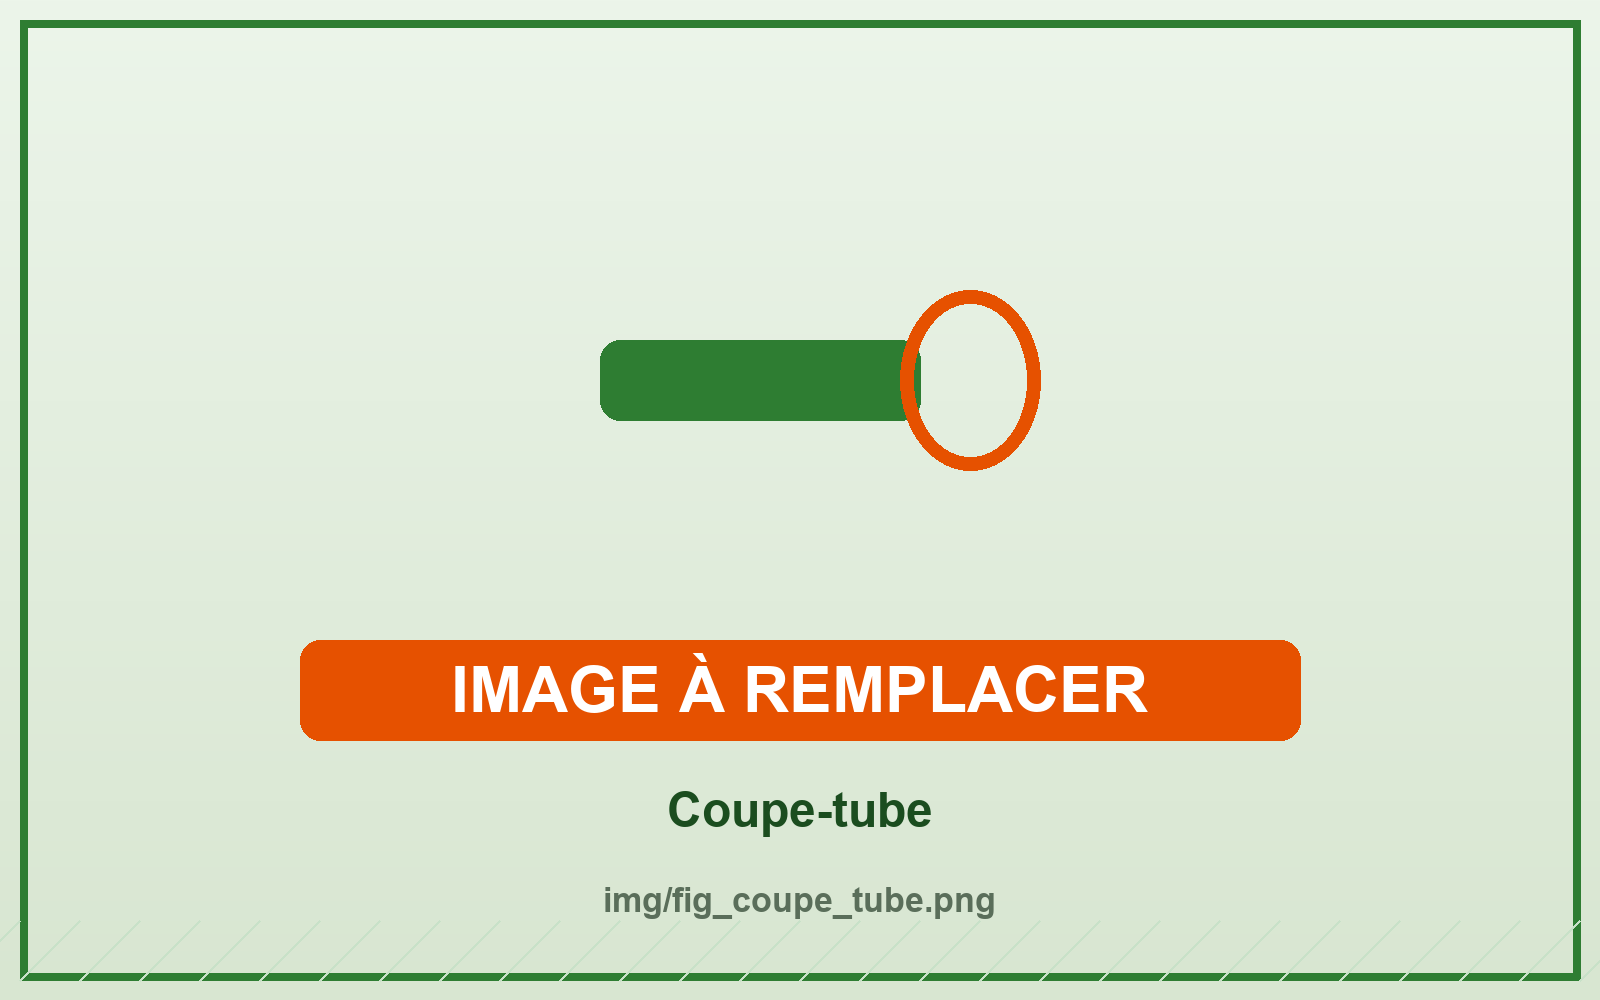
\includegraphics[width=\linewidth]{img/fig_coupe_tube}
  \caption{coupe-tube}\label{fig:coupetube}
\end{minipage}\hfill
\begin{minipage}{0.31\textwidth}\centering
  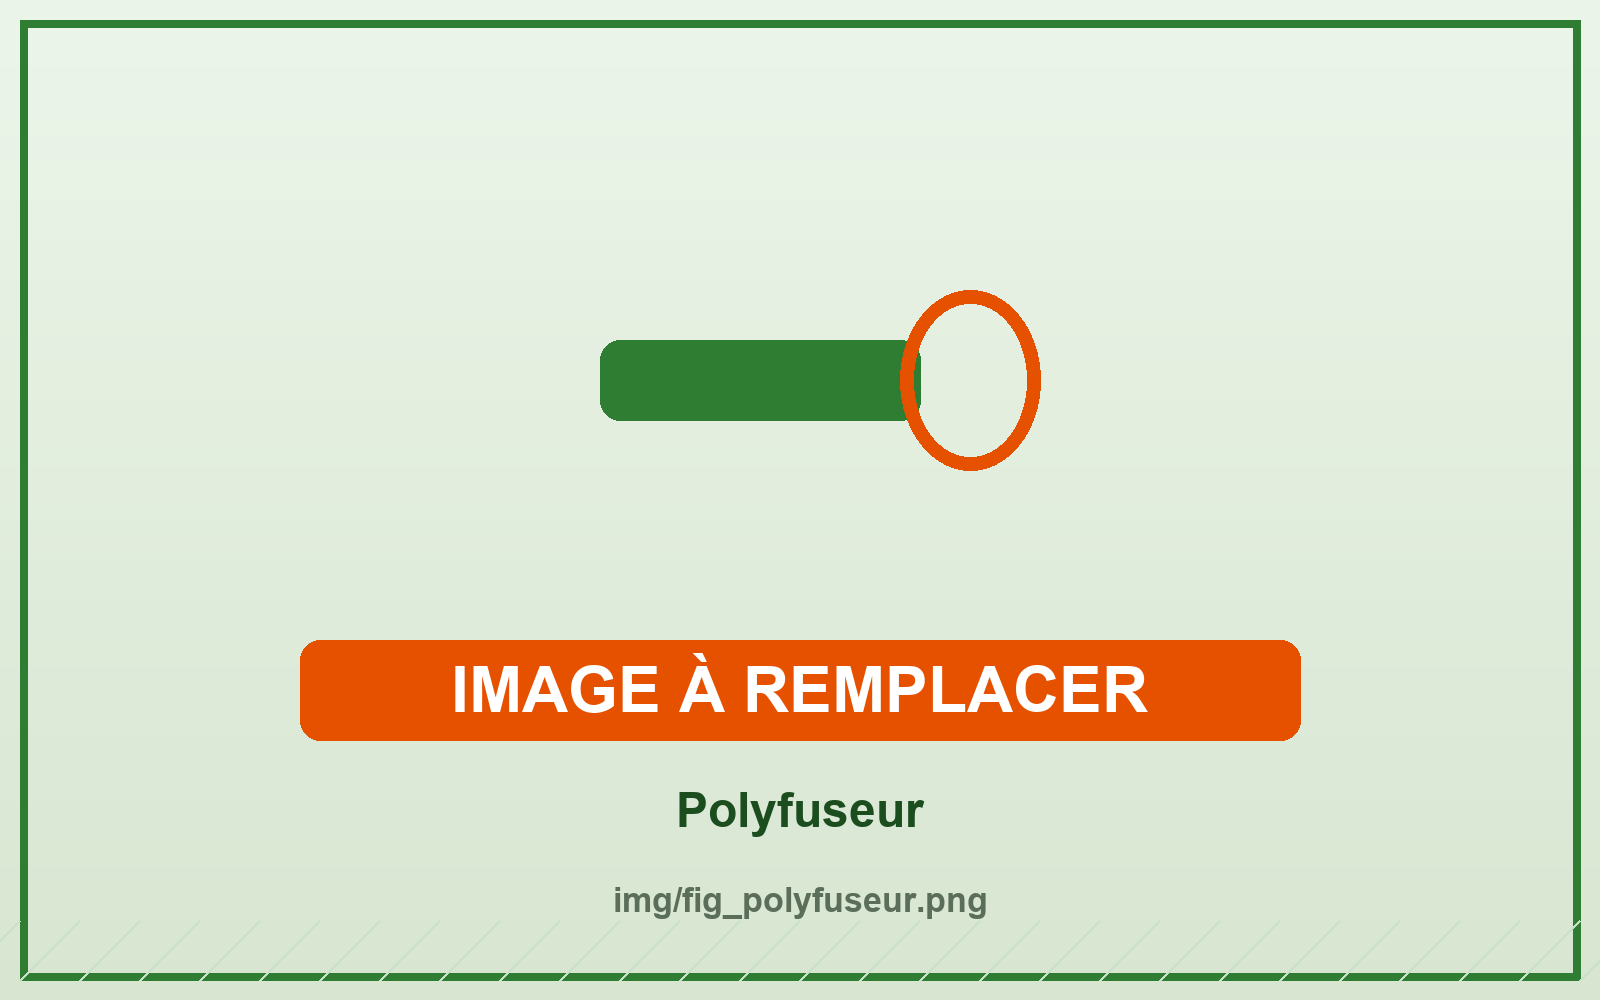
\includegraphics[width=\linewidth]{img/fig_polyfuseur}
  \caption{polyfuseur}\label{fig:polyfuseur}
\end{minipage}
\end{figure}

\begin{itemize}
  \item \textbf{Flexibles de raccordement} (figure~\ref{fig:flexible}) : en inox tressé, ils
        relient la canalisation fixe à la robinetterie des appareils.
  \item \textbf{Coupe-tube} (figure~\ref{fig:coupetube}) : il assure une coupe nette et
        perpendiculaire des tubes PPR de petit diamètre, condition d'une bonne soudure.
  \item \textbf{Polyfuseur} (figure~\ref{fig:polyfuseur}) : appareil chauffant équipé de
        matrices mâle et femelle, il permet d'assembler les tubes et raccords PPR par fusion,
        sans colle.
\end{itemize}

\section{Mise en œuvre : modes opératoires}

\subsection{Assemblage des tubes PPR par polyfusion}
La polyfusion soude le tube et le raccord en fondant simultanément leurs surfaces de contact.
La température de la matrice doit être de \SI{260}{\celsius} \cite{wavinPPR}. Le mode
opératoire est le suivant :
\begin{enumerate}
  \item monter les matrices du diamètre voulu et laisser le polyfuseur atteindre
        \SI{260}{\celsius}, en attendant quelques minutes après le voyant de température ;
  \item couper le tube d'équerre au coupe-tube, l'ébavurer et le nettoyer ;
  \item marquer sur le tube la profondeur d'emboîtement ;
  \item engager simultanément le tube et le raccord dans les matrices, sans rotation ;
  \item respecter le temps de chauffe indiqué par le fabricant pour le diamètre ;
  \item retirer les pièces et les emboîter immédiatement, sans rotation, jusqu'au repère ;
  \item maintenir l'assemblage quelques secondes, puis le laisser refroidir avant toute
        sollicitation.
\end{enumerate}
Un temps de chauffe trop court donne une soudure non étanche. Un temps trop long rétrécit le
passage intérieur par formation d'un bourrelet.

\subsection{Montage d'un réducteur de pression et d'un manomètre}
\begin{enumerate}
  \item isoler et vidanger le tronçon concerné ;
  \item repérer le sens d'écoulement indiqué par la flèche sur le corps du réducteur ;
  \item monter le réducteur entre deux vannes d'isolement, en amont de la distribution d'étage,
        avec un filtre en amont si le modèle n'en comporte pas ;
  \item assurer l'étanchéité des filetages au ruban PTFE ou à la filasse avec pâte ;
  \item visser le manomètre sur la prise prévue en aval (figure~\ref{fig:montage_reducteur}) ;
  \item remettre en eau lentement, puis régler la pression aval à la valeur prescrite
        (environ \SI{3}{bar}) en lisant le manomètre, robinets fermés.
\end{enumerate}

\figureimg{img/fig_reducteur_montage}{0.62\textwidth}{montage du réducteur de pression et du manomètre sur la distribution d'étage}{fig:montage_reducteur}

\subsection{Isolation des canalisations}
Les canalisations d'eau chaude sont isolées pour limiter les pertes de chaleur. Les
canalisations d'eau froide qui traversent des zones chaudes ou climatisées le sont pour éviter
la condensation. L'isolant utilisé est une mousse élastomère à cellules fermées (de type
Armaflex), qui forme également un pare-vapeur \cite{armacell}. Les manchons sont fendus,
posés sur le tube, puis collés à la colle néoprène sur toute la longueur de la fente et aux
jonctions, sans étirer le matériau (figure~\ref{fig:isolation}).

\figureimg{img/fig_isolation_pose}{0.62\textwidth}{pose de l'isolant à cellules fermées sur une canalisation}{fig:isolation}

\subsection{Essai d'étanchéité}
Avant de refermer les gaines et de poser les revêtements, chaque réseau est soumis à un essai
de pression conforme au NF DTU~60.1 et au cahier des charges du marché \cite{dtu601,ffbEssais}.
Sur le chantier, l'essai se déroulait ainsi :
\begin{enumerate}
  \item obturer toutes les extrémités et purger l'air du réseau ;
  \item monter en pression avec la pompe d'épreuve jusqu'à la pression d'essai prescrite ;
  \item isoler la pompe et relever la pression au manomètre ;
  \item maintenir l'essai pendant la durée prescrite, sans chute de pression ;
  \item inspecter visuellement chaque assemblage ;
  \item consigner le résultat sur la fiche d'autocontrôle (\hyperref[ann:fiche]{annexe~2}).
\end{enumerate}
La pression et la durée d'essai sont celles du cahier des charges : \AC{pression d'essai et
durée retenues sur le chantier}.

\section{Hygiène, sécurité et environnement}

Les travaux de plomberie sur un chantier de grande hauteur exposent à plusieurs risques :
chutes de hauteur, brûlures (polyfuseur à \SI{260}{\celsius}), coupures, manutention de charges
et risques électriques. Les mesures de prévention appliquées sont les suivantes :
\begin{itemize}
  \item port obligatoire des EPI : casque, chaussures de sécurité, gants, lunettes, et
        harnais pour les travaux en hauteur ;
  \item polyfuseur posé sur son support, jamais laissé sous tension sans surveillance ;
  \item escabeaux et échafaudages vérifiés avant usage ;
  \item rangement du poste de travail et évacuation quotidienne des chutes de tubes ;
  \item tri des déchets (plastiques, emballages) et récupération des chutes réutilisables.
\end{itemize}
Des photographies des EPI et du matériel d'essai figurent en \hyperref[ann:photos]{annexe~3}.

\section{Liens avec le froid et la climatisation}

Bien que le thème de ce rapport soit la plomberie sanitaire, plusieurs activités du stage
relèvent directement de notre spécialité.

\subsection{Isolation et condensation}
Lorsqu'une canalisation froide traverse un air chaud et humide, sa surface peut descendre
sous la \textbf{température de rosée} de l'air : la vapeur d'eau s'y condense, ce qui provoque
des gouttes, des taches et de la corrosion. C'est exactement le phénomène que l'on combat en
climatisation sur les lignes d'aspiration et les réseaux d'eau glacée. L'isolant à cellules
fermées maintient la surface extérieure au-dessus du point de rosée.

\subsection{Rappel du cycle frigorifique}
Les climatiseurs installés dans le bâtiment fonctionnent selon le cycle frigorifique à
compression de vapeur (figure~\ref{fig:cycle}). Le fluide frigorigène s'évapore dans
l'évaporateur en absorbant la chaleur de la pièce. Il est comprimé par le compresseur, se
condense dans le condenseur en rejetant cette chaleur à l'extérieur, puis se détend dans le
détendeur avant de revenir à l'évaporateur.

\begin{figure}[H]\centering
% Cycle frigorifique à compression de vapeur
\begin{tikzpicture}[font=\small, >=Stealth,
  org/.style={draw=vertnuit, fill=vertclair, rounded corners=3pt, align=center,
              minimum width=3.2cm, minimum height=1.1cm, font=\small\bfseries},
  hp/.style={red!75!black, line width=1.5pt, ->},
  bp/.style={blue!70!black, line width=1.5pt, ->}]
  \node[org] (cond) at (0,3) {Condenseur\\{\scriptsize\normalfont (unité extérieure)}};
  \node[org] (evap) at (0,0) {Évaporateur\\{\scriptsize\normalfont (unité intérieure)}};
  \node[org, minimum width=2.4cm] (comp) at (4.2,1.5) {Compresseur};
  \node[org, minimum width=2.4cm] (det) at (-4.2,1.5) {Détendeur};
  \draw[hp] (comp.north) |- node[pos=0.75, above] {vapeur HP, chaude} (cond.east);
  \draw[hp] (cond.west) -| node[pos=0.25, above] {liquide HP} (det.north);
  \draw[bp] (det.south) |- node[pos=0.75, below] {mélange BP, froid} (evap.west);
  \draw[bp] (evap.east) -| node[pos=0.25, below] {vapeur BP} (comp.south);
  \draw[->, orange!80!black, line width=1pt] (0,4.0) -- ++(0,0.8) node[above] {chaleur rejetée à l'extérieur};
  \draw[<-, teal, line width=1pt] (0,-0.6) -- ++(0,-0.8) node[below] {chaleur absorbée dans la pièce};
\end{tikzpicture}

\caption{cycle frigorifique à compression de vapeur}\label{fig:cycle}
\end{figure}

\subsection{Évacuation des condensats des climatiseurs}
L'eau condensée sur l'évaporateur des unités intérieures doit être évacuée. Les tuyaux de
condensats sont raccordés au réseau d'eaux usées par l'intermédiaire d'un \textbf{siphon},
qui empêche la remontée des odeurs, avec une pente régulière d'au moins 1 \%. Lors de notre
appui à l'équipe climatisation (semaine S15), nous avons participé à ces raccordements
(figure~\ref{fig:condensats}). Ils montrent concrètement l'interface entre les deux lots.

\figureimg{img/fig_condensats_split}{0.6\textwidth}{raccordement de l'évacuation des condensats d'une unité intérieure}{fig:condensats}

\subsection{Eau chaude sanitaire et pompe à chaleur}
La production d'eau chaude sanitaire peut être assurée par une \textbf{pompe à chaleur}, qui
utilise le même cycle frigorifique que le climatiseur, mais en valorisant la chaleur du
condenseur. Sur les bâtiments climatisés, la chaleur rejetée par les groupes peut même être
récupérée pour préchauffer l'eau chaude sanitaire. Cette solution réduit fortement la
consommation d'énergie.

\conclusionPartielle
La plomberie sanitaire d'un immeuble repose sur des règles précises de débit, de vitesse et de
pression. L'étude de cas montre que la colonne montante doit être dimensionnée pour le dernier
étage, et que les étages bas nécessitent des réducteurs de pression. La qualité de la mise en
œuvre (polyfusion, isolation, essais) conditionne la fiabilité de l'ouvrage. Enfin, ce thème
rejoint notre spécialité par l'isolation, les condensats et la production d'eau chaude. Ces
observations nourrissent les critiques et suggestions de la quatrième partie.
